\documentclass[output=paper,colorlinks,citecolor=brown            ,chinesefont]{langscibook}
\ChapterDOI{10.5281/zenodo.17158188}
\author{Angelika Kiss\orcid{0000-0001-8064-3687}\affiliation{University of Toronto} and Roger Yu-Hsiang Lo\orcid{0000-0003-3652-7384}\affiliation{University of British Columbia} and Justin R. Leung\orcid{0000-0003-4780-9424}\affiliation{University of Toronto}}
\title[Cantonese sentence-final particles \& rhetorical questions]{What can Cantonese sentence-final particles tell us about rhetorical questions?}
\abstract{Rhetorical questions have been analyzed both as utterances equivalent to assertions and as questions. We acknowledge that they have the characteristics of both: their hybrid nature is best captured if we give them an inquisitive semantic treatment. Rhetorical questions can suggest both an empty set answer and a non-empty set answer, and this fact gives rise to an asymmetry in terms of their inquisitiveness and informativity, which is also reflected in their prosody. In a perception experiment, Cantonese speakers associated information-seeking questions and rhetorical questions suggesting an empty set answer with a certain intonational contour on the sentence-final particle, but there was no clear pattern for rhetorical questions with a non-empty set answer. We explain this pattern by the informativity/inquisitiveness of these utterances, which maps to different levels of dependence from the common ground.}
  
%move the following commands to the "local..." files of the master project when integrating this chapter
\IfFileExists{../localcommands.tex}{%hack to check whether this is being compiled as part of a collection or standalone
   \usepackage{tabularx,multicol}
%	\setlength{\multicolsep}{6.0pt plus 2.0pt minus 2.0pt}
\usepackage{array} % for the 'm' column type
\usepackage{multirow}

%font:
\usepackage{siunitx}
\sisetup{group-digits=none}

\usepackage{textcomp} %emdash

%\usepackage{libertinus−otf}
%\setmainfont{Libertinus}

 
\usepackage{langsci-optional}
\usepackage{langsci-lgr}
\usepackage{langsci-gb4e}
\usepackage{langsci-basic}
\usepackage{langsci-affiliations}
\usepackage{langsci-branding}

\usepackage{url}
\urlstyle{same}
\usepackage{orcidlink}

%\usepackage{langsci-textipa}

\usepackage{amsmath}
\usepackage{amssymb}
\usepackage{stmaryrd}

%\usepackage{biblatex}%citation input! DO NOT CHANGE!
%\usepackage[american]{babel}
%\usepackage{csquotes}
%\usepackage[style=apa]{biblatex}
%\bibliographystyle{linquiry2}
%\usepackage[hidelinks, bookmarks=false, pdfstartview=FitH]{hyperref} %bookmarks=false, urlcolor=blue,

\usepackage{pifont} %checkmarks
%\usepackage{ulem}

%no new packages for 02.tex :

%\usepackage{setspace}
%\doublespacing
%\singlespacing


\usepackage{tikz-qtree}
\usepackage{tikz-qtree-compat}
\tikzset{every tree node/.style={align=center,anchor=north}}
%\usepackage{qtree,tree-dvips}%for trees, dvips won't work with figures unless figures are converted to .eps. make sure Typeset is set to "tex and DVI", not "pdftex" 
%\qtreecentertrue
\usepackage[linguistics]{forest}
\forestset{
fairly nice empty nodes/.style={
delay={where content={}
{shape=coordinate, for siblings={anchor=north}}{}},
for tree={s sep=4mm} }
            }


\usepackage[nameinlink]{cleveref} %for \Cref{}
% \usepackage{comment}
% \usepackage{color}
% \usepackage{subcaption}
\usepackage{subfigure}
% \usepackage{caption}
\usepackage{arydshln}

% \usepackage[scale=0.8]{FiraMono}

%\usepackage[export]{adjustbox}

%03.tex packages:
%\usepackage{linguex}%for examples

%04.tex packages:
\usepackage{cancel}
\usepackage{metre}
% \pagenumbering{roman}

%08.tex packages:
% \usepackage{xeCJK} %Chinese fonts
% \newfontfamily{\NotoSerifTC}{Noto Serif TC}
% \setCJKmainfont{Noto Serif TC}

   %for all .tex files (Affiliation setups):
\SetupAffiliations{ output in groups = false,
separator between two = {\bigskip\\},
separator between multiple = {\bigskip\\},
separator between final two = {\bigskip\\},
orcid placement=after
}

% ORCIDs in langsci-affiliations 
\definecolor{orcidlogocol}{cmyk}{0,0,0,1}
\RenewDocumentCommand{\LinkToORCIDinAffiliations}{ +m }
  {%
    \,\orcidlink{#1}%
  }

\makeatletter
\let\thetitle\@title
\let\theauthor\@author
\makeatother

\newcommand{\togglepaper}[1][0]{
   \bibliography{../localbibliography}
   \papernote{\scriptsize\normalfont
     \theauthor.
     \titleTemp.
     To appear in:
     E. Di Tor \& Herr Rausgeberin (ed.).
     Booktitle in localcommands.tex.
     Berlin: Language Science Press. [preliminary page numbering]
   }
   \pagenumbering{roman}
   \setcounter{chapter}{#1}
   \addtocounter{chapter}{-1}
}

\newbool{bookcompile}
\booltrue{bookcompile}
\newcommand{\bookorchapter}[2]{\ifbool{bookcompile}{#1}{#2}}

\newcommand{\cmark}{\ding{51}}%
\newcommand{\xmark}{\ding{55}}%

%for 01.tex:
\newcommand{\eval}[2]{\llbracket #1\rrbracket^{#2}}

%02.tex:
\newcommand{\smiley}{:)}

%03.tex:
\newcommand{\exa}{\ea}
%\renewcommand{\firstrefdash}{}%changes citations from, e.g., (2-a) to (2a)
\newcommand{\den}[2]{\ensuremath{\llbracket#1\rrbracket}\textsuperscript{\ensuremath{#2}}}
\newcommand{\citepos}[1]{\citeauthor{#1}'s (\citeyear{#1})}
\newcommand{\tp}[1]{\ensuremath{{\langle #1 \rangle}}}

\newcommand{\rise}{$\nearrow$\xspace}
\newcommand{\fall}{$\searrow$\xspace}
\newcommand{\notp}{\emph{not}-$p$\xspace}

%09.tex:
%\newcommand\den[1]{\ensuremath{[\![ #1 ]\!]}}
%\newcommand{\int}[1]{\ensuremath{\llbracket #1 \rrbracket}}

%13.tex:
\newcommand{\PreserveBackslash}[1]{\let\temp=\\#1\let\\=\temp}
% \newcolumntype{C}[1]{>{\PreserveBackslash\centering}p{#1}}
\newcolumntype{R}[1]{>{\PreserveBackslash\raggedleft}p{#1}}
\newcolumntype{L}[1]{>{\PreserveBackslash\raggedright}p{#1}}

\newcommand{\SB}{\textsubscript}
\newcommand{\SuB}{\textsuperscript}

\newcommand{\quotecite}[1]{\citeauthor{#1}'s (\citeyear*{#1})}

   %% hyphenation points for line breaks
%% Normally, automatic hyphenation in LaTeX is very good
%% If a word is mis-hyphenated, add it to this file
%%
%% add information to TeX file before \begin{document} with:
%% %% hyphenation points for line breaks
%% Normally, automatic hyphenation in LaTeX is very good
%% If a word is mis-hyphenated, add it to this file
%%
%% add information to TeX file before \begin{document} with:
%% %% hyphenation points for line breaks
%% Normally, automatic hyphenation in LaTeX is very good
%% If a word is mis-hyphenated, add it to this file
%%
%% add information to TeX file before \begin{document} with:
%% \include{localhyphenation}
\hyphenation{
    par-a-digm
}
\hyphenation{
que-stions
}
\hyphenation{
na-me-l-y
}
\hyphenation{
ge-ne-ra-tion
}
\hyphenation{
Hir-sch-berg}
\hyphenation{
stee-p-er
}
\hyphenation{
inter-ro-ga-tives
}
\hyphenation{
cons-truc-tion
}
\hyphenation{
p-u-sh-ed
}
\hyphenation{
A-mong
}
\hyphenation{
award-ed
}
\hyphenation{
synta-ctic
}
%\hyphenation{
%wh-ich
%}
\hyphenation{
call-ed
}
\hyphenation{
mo-no-po-lar
}
\hyphenation{
proso-dic
}
\hyphenation{
non-ve-ri-di-cal
}
\hyphenation{
Ro-me-ro
}
\hyphenation{
though
}
\hyphenation{
ra-ther
}
\hyphenation{
mo-da-li-ty
}
\hyphenation{
prag-ma-ti-cal-ly
}
\hyphenation{
trans-ver-sal
}
\hyphenation{
re-se-arch
}
\hyphenation{
clau-s-es
}
\hyphenation{
c-lau-se
}
\hyphenation{
spea-k-er
}
\hyphenation{
a-mon-g-st
}
\hyphenation{
th-rou-gh
}
\hyphenation{
ad-dres-see
}
\hyphenation{
mo-da-li-s-ed
}
\hyphenation{
Ja-mie-son}








\hyphenation{
    par-a-digm
}
\hyphenation{
que-stions
}
\hyphenation{
na-me-l-y
}
\hyphenation{
ge-ne-ra-tion
}
\hyphenation{
Hir-sch-berg}
\hyphenation{
stee-p-er
}
\hyphenation{
inter-ro-ga-tives
}
\hyphenation{
cons-truc-tion
}
\hyphenation{
p-u-sh-ed
}
\hyphenation{
A-mong
}
\hyphenation{
award-ed
}
\hyphenation{
synta-ctic
}
%\hyphenation{
%wh-ich
%}
\hyphenation{
call-ed
}
\hyphenation{
mo-no-po-lar
}
\hyphenation{
proso-dic
}
\hyphenation{
non-ve-ri-di-cal
}
\hyphenation{
Ro-me-ro
}
\hyphenation{
though
}
\hyphenation{
ra-ther
}
\hyphenation{
mo-da-li-ty
}
\hyphenation{
prag-ma-ti-cal-ly
}
\hyphenation{
trans-ver-sal
}
\hyphenation{
re-se-arch
}
\hyphenation{
clau-s-es
}
\hyphenation{
c-lau-se
}
\hyphenation{
spea-k-er
}
\hyphenation{
a-mon-g-st
}
\hyphenation{
th-rou-gh
}
\hyphenation{
ad-dres-see
}
\hyphenation{
mo-da-li-s-ed
}
\hyphenation{
Ja-mie-son}








\hyphenation{
    par-a-digm
}
\hyphenation{
que-stions
}
\hyphenation{
na-me-l-y
}
\hyphenation{
ge-ne-ra-tion
}
\hyphenation{
Hir-sch-berg}
\hyphenation{
stee-p-er
}
\hyphenation{
inter-ro-ga-tives
}
\hyphenation{
cons-truc-tion
}
\hyphenation{
p-u-sh-ed
}
\hyphenation{
A-mong
}
\hyphenation{
award-ed
}
\hyphenation{
synta-ctic
}
%\hyphenation{
%wh-ich
%}
\hyphenation{
call-ed
}
\hyphenation{
mo-no-po-lar
}
\hyphenation{
proso-dic
}
\hyphenation{
non-ve-ri-di-cal
}
\hyphenation{
Ro-me-ro
}
\hyphenation{
though
}
\hyphenation{
ra-ther
}
\hyphenation{
mo-da-li-ty
}
\hyphenation{
prag-ma-ti-cal-ly
}
\hyphenation{
trans-ver-sal
}
\hyphenation{
re-se-arch
}
\hyphenation{
clau-s-es
}
\hyphenation{
c-lau-se
}
\hyphenation{
spea-k-er
}
\hyphenation{
a-mon-g-st
}
\hyphenation{
th-rou-gh
}
\hyphenation{
ad-dres-see
}
\hyphenation{
mo-da-li-s-ed
}
\hyphenation{
Ja-mie-son}








    \bibliography{localbibliography}
    \togglepaper[23]
}{}

\begin{document}
\maketitle

\section{Introduction}

Both the meaning and the form of rhetorical questions have received much attention in the literature. As for their meaning, they were first considered in general to have ``the illocutionary force of an assertion of the opposite polarity from what is apparently asked'' \citep[201]{Han2002}. In this sense, Han's example in \xref{opposite}, when asked as a rhetorical question, means that everybody likes ice-cream. Since under this reading, the set of people who do not like ice-cream is empty, we refer to such rhetorical questions as \textit{empty set} rhetorical questions.

\begin{exe}
\ex\label{opposite} After all, who doesn't like ice-cream? \hfill \citep[12]{Caponigro+2007}
\end{exe}

Later, it has become clear that not all rhetorical questions denote such an empty set answer, a fact also acknowledged by \citet[fn 6]{Han2002}, because they can denote a non-empty set answer as well. Under such a reading, \xref{opposite} would be used in a context where it is common ground that someone, known to both the speaker and the addressee, does not like ice-cream. In subsequent studies, rhetorical questions are defined as questions with an obvious answer \citep{Rohde2006, Caponigro+2007, Biezma+2017}. In these accounts, the obviousness of the answer plays a major role, but not the kind of that obvious answer (i.e., empty set or non-empty set answer). Rhetorical questions therefore would form a homogeneous group.

Given the homogeneity in terms of meaning, we expect that rhetorical questions will also form a homogeneous group in terms of their prosody. This is implicitly assumed by \citet{Biezma+2017}, who refer to a ``characteristic (hard to pin down) rhetorical prosody'' that characterizes rhetorical questions regardless of the kind of answer they expect.

A number of recent production studies have shown that the prosody of empty set rhetorical questions indeed distinguishes them from information-seeking questions (see \citealt{Braun+2018} for German, \citealt{Dehe+2019} for English, \citealt{Dehe+2020} for Icelandic, and \citealt{Zahner+2020} for Mandarin). But since these studies do not consider the class of non-empty set rhetorical questions, they neither support nor challenge the assumption that the two types of rhetorical questions have the same prosodic form.

However, based on even more recent production experiments by \citet{Lo+2019} on Cantonese and \citet{Lo+2020} on Mandarin, we have reason to believe that the kind of answer rhetorical questions suggest plays a role in their semantics. When participants read the same interrogative in three different contexts -- one that gives the interrogative an information-seeking question reading, one that gives it an empty set rhetorical question reading, and one that gives it a non-empty set rhetorical reading -- the utterances show a three-way distinction in certain prosodic properties, a contrast that is not predicted by any of the above-mentioned accounts.

If the two kinds of rhetorical questions are marked differently in their form, both from each other and from information-seeking questions, it suggests that the two types of rhetorical questions differ in their semantics. This is the conclusion of \citet{Kiss+2021}, who offer an inquisitive semantic analysis that describes the three question types as expressing three distinct kinds of speaker commitment because they form a scale in terms of how informative/inquisitive they are. Namely, information-seeking questions are the least informative, and empty set rhetorical questions are the most informative among the questions on their scale, and non-empty set rhetorical questions are between them.

In this chapter, we test these claims by means of a perception experiment done with native speakers of Cantonese; participants hear string-identical interrogatives which all have their sentence-final particle \textit{aa\textsuperscript{3}} prosodically manipulated.\footnote{The numbers 1 and 3 indicate the lexical tone of the particles. 1 is high level, 2 is high rising, 3 is mid level, 4 is low falling, 5 is low rising, and 6 is low level. See \citet{Matthews+2011} for a detailed characterization of Cantonese tones.} The experiment allows us to test whether there is indeed a three-way prosodic distinction among these question types, and indirectly, it allows us to see if the three question types indeed form a scale in terms of their informativity / inquisitiveness, which maps onto different degrees of context-dependence, which in turn may affect how strongly speakers associate a certain contour with one or the other question type.

To our knowledge, ours is the first study to compare both empty set and non-empty set rhetorical questions to each other and to information-seeking questions in a perception experiment. As such, it contributes to what we know about rhetorical questions, and to what we know about intonation and the \textit{aa}-family of sentence-final particles in Cantonese.

The paper is organized as follows. In \sectref{sec:RQ}, we present arguments for the claim that rhetorical questions are questions, and distinguish empty set and non-empty set rhetorical questions. In \sectref{sec:inqsem}, we present \quotecite{Farkas+2017} inquisitive semantic analysis of questions and extend it following \citet{Kiss+2021} so that it comprises information-seeking and rhetorical wh-questions. \sectref{sec:Cantonese} presents previous work on the prosody of rhetorical questions, including Cantonese ones. In \sectref{sec:perception}, the perception experiment is described, which is followed by the general discussion in \sectref{sec:discussion} and by the conclusion in \sectref{sec:conclusion}.

\section{Rhetorical questions}
\label{sec:RQ}

In \sectref{subsec:questions}, we argue that rhetorical questions are better treated as (biased) questions, as opposed to assertions, and in \sectref{subsec:alike}, we show subtypes of rhetorical questions which differ in their meaning.

\subsection{Rhetorical questions as questions}
\label{subsec:questions}

It is widely known that rhetorical questions behave differently from genuine or information-seeking questions in discourse, namely they exhibit quite a few properties typically associated with assertions. Using the tests of \citet{Sadock1971,Sadock1974}, who differentiates what he calls ``queclaratives'' from information-seeking questions, \citet{Han2002} showed that rhetorical questions, but not information-seeking ones, can be introduced by \textit{after all} and can be followed by an utterance that is introduced by \textit{yet}. 

\begin{exe}
\ex\label{Sadock} 
\begin{xlist}
\ex\label{Sadock1} \textit{After all}, do phonemes have anything to do with language?
\ex\label{Sadock2} Do phonemes have anything to do with language? \textit{Yet} people continue to believe in them. \hfill \citet[225]{Sadock1971}, cited by \citet{Han2002}
\end{xlist}
\end{exe}

\textit{After all} and \textit{yet} can felicitously occur in assertions, but not in information-seeking questions; yet when the interrogative \textit{Do phonemes have anything to do with language?} is interpreted as a rhetorical question, it can appear in such environments.

Another assertion-like property rhetorical questions exhibit is their compatibility with strong negative polarity items or minimizers \citep{Han2002, Abels2003, Guerzoni2004, Biezma+2017}.

\begin{exe}
\ex\label{min} When did John \textit{lift a finger} to help us?
\end{exe}

Minimizers are felicitous in assertions but not in information-seeking questions. The interrogative in \xref{min} can only have a rhetorical question interpretation, conveying that `John never helped us'; thus rhetorical questions behave like assertions in this respect as well. 

These and further arguments gave rise to the view that rhetorical questions are assertions \citep{Han2002}, a view that has been challenged by the observations of \citet{Rohde2006} and \citet{Caponigro+2007}. The latter authors pointed out some inherently question-like properties of rhetorical questions that receive no explanation if they are treated as assertions. 

Most importantly, rhetorical questions can also suggest a non-empty answer as shown in \xref{RQ+}, not necessarily an empty set answer as in examples \xref{Sadock} and \xref{min}. 

\begin{exe}
\ex\label{RQ+} Who has fed you and given you a proper education?\\
(Context: a mother to her son) \hfill \citet{Rohde2006} citing \citet{Han1998}
%\ex\label{RQ+2} Situation: Mina helped Luca when he was in trouble and both the Speaker and the Addressee are aware of that. Now Luca adores Mina for helping him.\\
%\textsc{Speaker}: It's understandable that Luca adores Mina. After all, who helped him when he was in trouble?\\
%\textsc{Addressee} or \textsc{Speaker}: Mina / \#Nobody \hfill \citep{Caponigro+2007}
%\end{xlist}
\end{exe}

In addition, rhetorical questions can be answered the same way as questions, regardless of the kind of answer they suggest, as shown by the following minimal pair in \xref{answerhood}.

\begin{exe}
\ex\label{answerhood}
\begin{xlist}
\ex\label{answerhood1} \textsc{Speaker:} You should stop saying that Luca didn't like the party last night. \textit{After all,
who was the only one that was still dancing at 3am?}\\
\textsc{Addressee} or \textsc{Speaker:} Luca.
\ex\label{answerhood2} \textsc{Speaker:} You should stop saying that Luca didn't like the party last night. \textit{After all,
Luca was the only one that was still dancing at 3am!}\\
\textsc{Addressee} or \textsc{Speaker:} \#Luca. \hfill \citep[124]{Caponigro+2007}
\end{xlist}
\end{exe}

If rhetorical questions function as assertions, they should be felicitous as answers to information-seeking questions, as in \xref{answer1}, but this is not always the case, as \citet{Biezma+2017} point out. 

\begin{exe}
\ex\label{answer}
\begin{xlist}
\ex\label{answer1} A: Does Ed McMahon drink?\\
B: Is the Pope a Catholic? \hfill \citep[438]{Schaffer2005}
\ex\label{answer2} A: Does Mother Teresa drink? \\
B: \#Does Mother Teresa drink? (as a rhetorical question)
\end{xlist}
\end{exe}

While A receives an affirmative answer from B in \xref{answer1} who uses the rhetorical reading of \textit{Is the Pope a Catholic?}, \xref{answer2} shows that if both the information-seeking question and the rhetorical question given in response are conveyed by the same interrogative, the result is odd. B's utterance in \xref{answer2} can at most be interpreted as an echo question, but not a rhetorical question conveying `Mother Teresa does not drink', which, under the assertion-like analysis, should be an acceptable answer. 

However, if we consider the proposal of those who treat rhetorical questions as questions with an obvious answer \citep{Rohde2006, Caponigro+2007, Biezma+2017}, the infelicity of \xref{answer2}-B receives a natural explanation. Speaker A raised the issue of whether Mother Teresa drinks, after which B's response is infelicitous for two reasons. First, because B's utterance is a question, too, so despite the obvious answer, it still raises the same issue, which is an infelicitous move. Second, since A's utterance is an information-seeking question, it is evidence that the issue of `whether Mother Teresa drinks' is not settled. If so, the answer to B's utterance should not be treated as common ground.

Treating rhetorical questions as questions with an obvious answer has further advantages. Unlike in the assertion-like analysis, both rhetorical questions suggesting an empty set answer and ones with a non-empty set answer are included; and it explains why rhetorical questions can be answered. Lastly, \citet{Caponigro+2007} point out that rhetorical questions are also like information-seeking questions in that they can have multiple wh-phrases and they can also be embedded.

However, the question-like analysis cannot explain why minimizers can occur in rhetorical questions if the suggested answer is the empty set, to which the assertion-like analysis offers a solution. We nevertheless adopt a question-like analysis of rhetorical questions, and propose that to account for their assertion-like properties, we need to take into account the kind of answer suggested by the utterance (i.e., whether it is an empty set answer or a non-empty answer). 
%The fact that both views on rhetorical questions capture true and important facts calls for a suspension of the assertion/question dichotomy.

\subsection{Rhetorical questions are not all alike}
\label{subsec:alike}

Rhetorical questions thus can convey an empty set answer or a non-empty set answer, as shown in examples \xref{empty2} and \xref{nonempty2}, respectively; however, this distinction does not play a role in the analyses that treat them as questions \citep{Rohde2006, Caponigro+2007, Biezma+2017}. 

\begin{exe}
\ex\label{empty} Context: David is considering helping his colleagues.
\begin{xlist}
\ex\label{empty1} David: Should I help them? 
\ex\label{empty2} Erez: No way! Who helped you when you were in trouble?
\end{xlist}
\ex\label{nonempty} Context: It is common ground that Cleo helped David when he was in trouble.
\begin{xlist}
\ex\label{nonempty1} David: Who should I trust? 
\ex\label{nonempty2} Erez: Well, who helped you when you were in trouble? (Of course Cleo!)
\end{xlist}
\end{exe}


The only exception known to us is the account of \citet{Jamieson2018phd}, who treats the two rhetorical question types differently. \citet{Jamieson2018phd} refers to empty set rhetorical questions as \textit{generic} rhetorical questions. This generic interpretation is due to a metavariable $\epsilon$, which affects the semantic value of the wh-phrase so that it no longer denotes the ordinary type of domain it is associated with, that is, \textit{who} does not denote humans, \textit{where} does not denote locations, etc. \xref{metavariable}. The metavariable guarantees that the answer set becomes empty under its ordinary value, and so the rhetorical question is interpreted as an assertion, as in Han's approach. Thus, Erez's utterance in \xref{empty2} amounts to saying `Nobody helped you when you were in trouble'.

\begin{exe}
\ex\label{metavariable} 
\begin{xlist}
\ex\label{metavar1} $\llbracket$who$\rrbracket$$^o$ = $\lambda$$w$.$\epsilon$ $\notin$ human in $w$
\ex\label{metavar3} $\llbracket$where$\rrbracket$$^o$ = $\lambda$$w$.$\epsilon$ $\notin$ location in $w$
\hfill \citep[324]{Jamieson2018phd}
\end{xlist}
\end{exe}

Rhetorical questions that suggest a non-empty answer, on the other hand, are referred to by Jamieson as \textit{pragmatic} rhetorical questions: these are questions which owe their assertion-like properties to the context, as they are questions with an already known answer. In agreement with \citet{Jamieson2018phd}, we posit that the two types of rhetorical questions have distinct semantics.

\section{Rhetorical questions in inquisitive semantics}
\label{sec:inqsem}

Previous analyses of rhetorical questions have made it clear that this question type shares several characteristics with assertions, as well as with information-seeking questions. Rhetorical questions are not the only question type with both assertion-like and question-like properties. Tag questions, consisting of a declarative anchor and a reduced interrogative clause, have been analyzed as a hybrid speech act type, being an assertion and a question at the same time, and declarative questions (also known as rising declaratives), which consist of a declarative clause and bear a question-like intonation, share properties of both as well \citep{Gunlogson2003, Asher+2007, Farkas+2017}. 

The way \citet{Farkas+2017} analyze such non-canonical questions is particularly important for our purposes because the inquisitive semantic framework they use makes it possible to capture both their assertion-like and question-like nature. In addition, they make falsifiable claims about the contribution of the marked form to utterance meaning. 

We are primarily interested in wh-interrogatives. This is because, polar interrogatives suggesting a positive answer, which would correspond to rhetorical questions with a non-empty set answer, proved to be considerably more problematic to elicit in experiemntal settings. That is, in experimental settings, these were much harder to elicit than ones that suggest the empty set as an answer. 
%We are primarily interested in wh-interrogatives, because polar interrogatives suggesting a positive answer (which would be the counterpart of rhetorical questions with a non-empty set answer) proved to be considerably more problematic to elicit in experimental settings than ones that suggest the empty set as an answer. 
Polar rhetorical questions suggesting a positive answer nevertheless do exist, as \citet{Rohde2006} reports, a corpus example of which is shown in \xref{polar+}.

\begin{exe}
\ex\label{polar+} Has the educational system been so watered down that anybody who's above average is now gifted? \citep[135]{Rohde2006}
\end{exe}

While \citet{Farkas+2017} only treat utterance types with a sentence radical, they claim that wh-interrogatives, too, can fit in their model. In this paper, we adopt the proposal of \citet{Kiss+2021} (see \sectref{subsec:genrec}) who offer an extension of their inquisitive semantic framework to accommodate wh-interrogatives conveying information-seeking and rhetorical questions, but our claims arguably also hold for polar interrogatives.

\subsection{Inquisitive semantics}

\subsubsection{Basic notions}
\label{subsubsec:basic}

In \citet{Farkas+2017}, a proposition $P$ is modeled not only as a set of possible worlds \citep{Stalnaker1978} but also as a set of information states, which themselves are sets of possible worlds. Besides their inquisitive content, propositions are also characterized by their informative content, marked as info($P$), which is a set of those possible worlds that are members of any of the information states within the given proposition. The inquisitive content of a proposition expresses the issue it raises, and the informative content expresses which possible worlds, if any, can be discarded from the speaker's commitment set.

%\begin{exe}
%\ex\label{prop} A proposition $P$ is a non-empty, downward closed set of information states 
%\begin{xlist}
%\ex\label{prop1} Inquisitive content:  the issue %embodied by $P$, resolved in a state s (or a substate $t$ of it) s. t. $s$ $\in$ $P$
%\ex\label{prop2} Informative content: For any %proposition $P$, info($P$) := $\bigcup$$P$
%\end{xlist}
%\end{exe}

Any information state $s$ can have a substate $t$ such that if a possible world is a member of $t$, it is also a member of $s$. Substates within an information state form a lattice, and their maximal element is referred to as an alternative. Whenever the possible worlds that make up a proposition $P$'s informative content do not form a single alternative, which would be a member of $P$'s inquisitive content, $P$ is inquisitive. And whenever the informative content of $P$ is a proper subset of the set of all possible worlds $W$, $P$ is informative. 

\begin{exe}
\ex\label{inqdef} Informative and inquisitive propositions
\begin{xlist}
\ex\label{inqdefa} A proposition $P$ is inquisitive iff info($P$) $\notin$ $P$
\ex\label{inqdefb} A proposition $P$ is informative iff info($P$) $\neq$ $W$
\hfill \citep[23]{Ciardelli+2018}
\end{xlist}
\end{exe}

A declarative sentence conveying an assertion consists of one alternative and is therefore informative and non-inquisitive, whereas a polar interrogative conveying an information-seeking question consists of two alternatives, and is therefore inquisitive and non-informative. Both assertions and polar questions have sentence radicals, which we assume, following \citet{Stenius1967}, is the part of a declarative or interrogative sentence that signifies its ``descriptive content''. Utterances with a sentence radical have what \citet{Farkas+2017} call a highlighted alternative, marked by \textbf{$\alpha$}, which is the alternative denoted by the sentence radical.

\begin{exe}
\ex\label{intdecI} Inquisitive and informative content of a declarative conveying an assertion 
\begin{xlist}
\ex\label{intdec1} $P$ = \{\textbf{$\alpha$}\}$^{\downarrow}$
\ex\label{intdec2} info($P$) = info($\alpha$)
\end{xlist}
\ex\label{intdecII} Inquisitive and informative content of a polar interrogative conveying an information-seeking question
\begin{xlist}
\ex\label{intdec3} $P$ = \{\textbf{$\alpha$}, $\overline{\alpha}$\}$^{\downarrow}$
\ex\label{intdec4} info($P$) = $W$
\end{xlist}
\end{exe}

The basic discourse context proposed by \citeauthor{Farkas+2017} keeps track of the participants, the table, and the commitment sets assigned to each participant, as outlined in \xref{context}.

\begin{exe}
\ex\label{context} A basic discourse context is a triple $\langle$\textsc{participants, table, commitments}$\rangle$, where:
\begin{xlist}
\ex\textsc{Participants}: the set of discourse participants;
\ex\textsc{Table}: a stack of propositions, representing the proposals made so far;
\ex\textsc{Commitments}: a function that maps every participant $x$ $\in$ \textsc{Participants} to a set of possibilities, those possibilities that $x$ is publicly committed to. \jambox*{\citep[255]{Farkas+2017}}
\end{xlist}
\end{exe}

``The common ground'' is the locus of mutual commitments \citep{Stalnaker1978, Farkas+2010}, which here is derived from the participants' commitment sets. %It is defined as ``the smallest set of possible worlds $s$ such that all discourse participants are publicly committed to the actual world being contained in $s$''.

\begin{exe}
\ex\label{def}
\begin{xlist}
\ex\label{def1} Commitment set: $cs_x = \bigcap\textsc{Commitments}(x)$
\ex\label{def2} Common ground: $cg = \bigcup\{cs(x) | x\in \textsc{Participants}\} $\\
\jambox*{\citep[255]{Farkas+2017}}
\end{xlist}
\end{exe}

\subsubsection{Semantic interpretation} 
\label{subsubsec:interpretation}

The elegance of \quotecite{Farkas+2017} account lies in differentiating what they refer to as the basic conventional discourse effects from the special discourse effects of an utterance, which is summarized by the division of labor principle.

\begin{exe}
\ex\label{Labor} Division of labor principle
\begin{xlist}
\ex\label{Labor1} The discourse effects of unmarked forms should be fully determined by their semantic content and the basic convention of use, $F_b$.
\ex\label{Labor2} The discourse effects of marked forms should always include the discourse effects that are dictated by their semantic content and the basic convention of use $F_b$. In addition, they may include special discourse effects connected to the particular sentence type involved. \\ \hfill \citep[250]{Farkas+2017}
\end{xlist}
\end{exe}

According to the division of labor principle, declaratives and interrogatives are interpreted by the same principle, and any differences in their interpretation arise from differences in their semantic content. The inquisitive content of utterance $\phi$ is added to the \textsc{Table} and its informative content, to \textsc{Commitments}$_x$.

\begin{exe}
\ex\label{Convention} Basic convention of use\\
If a discourse participant $x$ utters a declarative or interrogative sentence $\phi$, the discourse context is affected as follows:
\begin{xlist}
\ex The proposition expressed by $\phi$, $\llbracket\phi\rrbracket$, is added to the \textsc{Table}.
\ex The informative content of $\phi$, $\bigcup \llbracket \phi \rrbracket$, is added to \textsc{Commitments}$_x$.\\ \citep[265]{Farkas+2017}
\end{xlist}
\end{exe}

In the case of a declarative assertion, the \textsc{Table} is updated by an expression consisting of a single alternative, whereas a polar interrogative conveying an information-seeking question places both the highlighted alternative ($\alpha$) and its complement ($\overline{\alpha}$), on the \textsc{Table}. The speaker's commitments are updated by a set of worlds compatible with the alternative(s) on the \textsc{Table}, that is, with $\alpha$ in the case of an assertion, and with $W$ in the case of a polar interrogative. 

\begin{exe}
\ex\label{ConvA} Conventional discourse effects of $x$ uttering an assertion:
\begin{xlist}
\ex\label{ConvA1} \{$\alpha$\}$^\downarrow$ is added to the \textsc{Table} 
\ex\label{ConvA2} $\alpha$ is added to \textsc{Commitments}$_x$ 
\end{xlist}
\ex\label{ConventionPQ} Conventional discourse effects of $x$ uttering a polar question:
\begin{xlist}
\ex \{$\alpha, \overline{\alpha}$\}$^\downarrow$ is added to the \textsc{Table}
\ex \textit{W} is added to \textsc{Commitments}$_x$ \hfill \citep[266--267]{Farkas+2017}
\end{xlist}
\end{exe}


Marked utterances come with special discourse effects in addition to the basic conventional ones. In the case of utterance types with a highlighted alternative, the meaning added by the markedness conveys the level of credence the speaker has in the truth of the highlighted alternative. One way to add special discourse effects to an utterance is by marked intonation.  

\subsubsection{Boundary tones}
\label{subsec:boundary}

Special discourse effects do not arise arbitrarily; they are inherently tied to intonation. In marked utterance types such as declarative questions and tag questions, \citet{Farkas+2017} claim that sentence-final tunes play a crucial role in determining these special effects.

\begin{exe}
\ex\label{intonation} The contribution of sentence-final tunes to the special discourse effects of utterances
\begin{xlist}
\ex\label{intonation1} $\uparrow \: \: \: \rightsquigarrow$ zero to low credence
\ex\label{intonation2} $\downarrow \uparrow \: \rightsquigarrow$ moderate to high credence
\ex\label{intonation3} $\downarrow \downarrow \: \rightsquigarrow$ high credence \hfill  \citep[272]{Farkas+2017}
\end{xlist}
\end{exe}

At least in English utterances, the speaker marks high or low credence in the truth of the highlighted alternative by a falling and a rising sentence-final tune, respectively. The association of rises with low credence and of falls with high credence is in alignment with intuitions presented in earlier theoretical work on intonational contours and is also supported by empirical work, according to which sentence-final rising tunes are cross-linguistically associated with uncertainty and questionhood, while falling final tunes are associated with certainty and assertivity \citep{Pierrehumbert+1990, Gussenhoven+2000, Gussenhoven2004}. In sum, markedness in form entails markedness in meaning, and in addition, markedness in form maps systematically to markedness in meaning.

%\citet{Pierrehumbert+1990} claim that rises signal that an utterance is to be interpreted ``with respect to subsequent utterances''. Questions, among other things, qualify as utterances which depend on subsequent utterances (i.e., on an answer). At the same time, utterance-final falls indicate ``completeness'', that is, the utterance is ready for interpretation in itself, and it does not rely on subsequent utterances. Reliance on subsequent utterances in interpretation is a property that shows itself most prototypically in questions, and completeness, in assertions.

\subsection{Information-seeking and rhetorical wh-questions}
\label{subsec:genrec}

Wh-interrogatives do not have a highlighted alternative but a highlighted property \citep{Farkas2020}.\footnote{See also \citet{Roelofsen+2015}.} Following \citeauthor{Ciardelli+2017}'s \citeyearpar{Ciardelli+2017} composition rules, applying \textit{who} to the highlighted property yields a set of alternatives that correspond to a Hamblin-set \citep{Hamblin1973}, which we label $\Alpha$ (capital $\alpha$). Consider the following interrogative. 

\begin{exe}
\ex\label{wh} Who helped David?
\end{exe}

Let the domain of \textit{who} in \xref{wh} consist of Ann, Ben and Cleo. In this context, $\Alpha$ = \{`Ann helped David', `Ben helped David', `Cleo helped David'\}. $\Alpha$ thus consists of three alternatives.

We propose that the basic conventional discourse effects of a wh-interrogative conveying an information-seeking question consist of the same two components as those of other utterances considered so far: the \textsc{Table} is updated by the inquisitive content of the utterance, and \textsc{Commitments}$_S$, the speaker's commitment set is updated by its informative content. The inquisitive content of a wh-interrogative is $P$, an inquisitive proposition, consisting of the alternatives that are elements of ($\Alpha$ $\cup$ $\overline{\Alpha}$). And the informative content of a wh-question is $W$, just like in the case of polar interrogatives. 

%They place more than one alternatives (i.e., an inquisitive proposition) on the table, which makes them inquisitive, and since the alternatives together cover logical space, there is no possible world they discard, hence they are not informative. 

\begin{exe}
\ex\label{whISQ} Basic conventional discourse effects of an information-seeking question
\begin{xlist}
\ex\label{whISQ1}  $\Alpha^\downarrow\cup\overline{\Alpha}$$^\downarrow$ is added to the \textsc{Table}
\ex\label{whISQ2} $W$ is added to \textsc{Commitments}$_S$.
\end{xlist}
\end{exe}

Note that (\ref{whISQ}) applies to polar interrogatives as well; only 
($\Alpha\cup\overline{\Alpha}$) is a set consisting of only two alternatives \{$\alpha, \overline{\alpha}$\}, since both $\Alpha$ and $\overline{\Alpha}$ are singletons.

Rhetorical questions have the same basic conventional discourse effects as information-seeking questions, but we propose, along with \citet{Jamieson2018phd}, that empty set and non-empty set rhetorical questions are both marked in meaning in their own way. Rhetorical questions that suggest a non-empty answer signal that the actual world is a member of an information state found within $\Alpha$, and rhetorical questions suggesting an empty set as their answer signal that the actual world is to be found in $\overline{\Alpha}$.

As for rhetorical questions with a non-empty set answer, the message the addressee receives is that the answer to the question is already known, and it is some member(s) from the domain denoted by the wh-phrase. But the addressee still needs to ``consult'' the common ground and the alternatives in $\Alpha$ in order to arrive at the intended interpretation of the utterance. The special effect of a non-empty set rhetorical question is shown in (\ref{whRQ+E}).

\begin{exe}
\ex\label{whRQ+E} Special effect of a rhetorical question with a non-empty answer: \\
Instead of $W$, only info($\Alpha$) $\cap$ $cg$ is added to \textsc{Commitments}$_S$\footnote{\textit{Addition} in this case does not mean adding new information, because whatever is in \textit{cg} must by definition already be present in all interlocutors' commitments. We use addition in a wider sense, one that includes reading or underlining a certain piece of information. Interlocutors' beliefs and commitments may be steady over time, but this does not mean that these pieces of information are equally accessible to them at all times \citep{Clark1996}. Reminding someone of something they already have committed to therefore is a plausible discourse move, and we treat it as a special case of addition.}
\end{exe}

Consider again the example domain consisting of Ann, Ben and Cleo, and assume that `Cleo helped David' is common ground. If the addressee hears \textit{Who helped you when you were in trouble?}, they will understand that the answer is already common ground and that it is to be found within $\Alpha$, but the utterance alone does not encode which member of $\Alpha$ the answer is, so the addressee needs to find out which information states in $\Alpha$ conform to the common ground. Therefore, \textsc{Commitments}$_S$ is updated by only those worlds that are compatible with both $\Alpha$ and the $cg$. Thus the entire set of alternatives ($\Alpha\cup\overline{\Alpha}$) is put on the \textsc{Table} just as in the case of information-seeking questions \xref{whRQ+shrink1}, but the speaker's commitments get updated only by the intersection of $\Alpha$ and the common ground \xref{whRQ+shrink2}. 

\begin{exe}
\ex\label{whRQ+shrink} The discourse effects of rhetorical questions with a non-empty answer
\begin{xlist}
\ex\label{whRQ+shrink1} \textsc{Table}: $\Alpha$$^\downarrow$ $\cup$ $\overline{\Alpha}$$^\downarrow$
\ex\label{whRQ+shrink2} \textsc{Commitments}$_S$: info($\Alpha$) $\cap$ $cg$
\end{xlist}
\end{exe}

Assuming that the speaker takes it as common ground that Cleo helped David (an alternative we will label as $\gamma$), the addressee is invited to infer the following:

\begin{exe}
\ex\label{whRQ+shrink3} \textit{cg} $\cap$ info($\Alpha$) = $\gamma$
\end{exe}

\noindent If $\gamma$ is a member of the addressee's version of the common ground as well, the rhetorical question will likely achieve its communicative goal of underlining the fact represented by $\gamma$.

Given the definitions of inquisitiveness and informativity in \xref{inqdef}, a rhetorical question that suggests a non-empty answer set is both inquisitive and informative. It is inquisitive by virtue of its form: as an interrogative sentence, it updates the \textsc{Table} by a (non-empty and non-singleton) set of information states. The utterance is also informative because the informative content of the expression, due to the special effects \xref{whRQ+shrink2}, is a proper subset of $W$.

Rhetorical questions with an empty set answer convey that the answer is in the common ground, and that it is the empty set. The basic discourse effects of such rhetorical questions are the same as the ones of any question: they put the union of $\Alpha$ and its complement on the \textsc{Table}, and they update \textsc{Commitments}$_S$ by $W$. And their special discourse effects restrict the set of possible worlds that update \textsc{Commitments}$_S$ to only those that are members of info($\overline{\Alpha}$). 

\begin{exe}
\ex\label{whRQ-E} Special effect of a rhetorical question with an empty set answer: \\
Instead of $W$, only info($\overline{\Alpha}$) $\cap$ $cg$ is added to \textsc{Commitments}$_S$
\end{exe}

Again, the expression on the \textsc{Table} is the same as in the case of any question: the set consisting of all the alternatives that are members of $\Alpha$ or $\overline{\Alpha}$. However, \textsc{Commitments}$_S$ does not get updated with the worlds compatible with all of these alternatives, only by the ones compatible with the empty set alternative. 

\begin{exe}
\ex\label{excont} 
\begin{xlist}
\ex\label{excont1} \textsc{Table}: $\Alpha$$^\downarrow$ $\cup$ $\overline{\Alpha}$$^\downarrow$
\ex\label{excont2} \textsc{Commitments}$_S$: info($\overline \Alpha$) $\cap$ $cg$ =  info($\overline{\Alpha}$) 
\end{xlist}
\end{exe}

$\overline{\Alpha}$ gets intersected with the common ground, and since $\overline{\Alpha}$ contains just one alternative,  \textsc{Commitments}$_S$ gets updated by an informative expression. 

The two types of rhetorical questions differ crucially in their interpretation. To interpret an empty set rhetorical question, the addressee may or may not rely on the common ground, because across contexts, regardless of whether $\overline{\Alpha}$ gets intersected with the $cg$ or not, the result is the same. As a consequence, a rhetorical question with an empty set answer can be interpreted correctly (i.e., according to the speaker's intentions) even in a defective context, where the addressee does not share the relevant piece of information that the speaker assumes to be common ground. In this sense, rhetorical questions with an empty set answer are less context-dependent than the ones with a non-empty set answer. To interpret a non-empty set rhetorical question, considering the common ground is crucial, as without it, the addressee is not able to understand what the speaker intended to say.\footnote{As a reviewer notes, it is possible to misinterpret the given rhetorical question, for example, it could happen that a speaker uses an empty set rhetorical question but the addressee interprets it as a non-empty set rhetorical question. Such a scenario can ensue in case of a defective context. If a non-empty set answer is given to a rhetorical question that the speaker said in order to suggest an empty set answer, that non-empty set answer will prove to the speaker that their common ground is not the same. Resolving the issue can happen in a variety of ways, an example of which is to address it explicitly. We only consider ideal cases of conversation (i.e., with contexts where interlocutors actually share the common ground), but we acknowledge that this phenomenon is pervasive enough to be accounted for in discourse models.}

This asymmetry is not predicted by previous question-like analyses of rhetorical questions, which treat them as a homogeneous utterance type. \citet{Biezma+2017} propose that rhetorical questions immediately resolve the question under discussion they raise, with which we agree; however, following \citet{Jamieson2018phd}, we argue that this resolution is achieved differently in the two cases, and the root of the asymmetry lies in the kind of answer that is suggested by the rhetorical question. 

\subsection{Gradient inquisitiveness}
\largerpage[2]
\label{subsec:gradient}

Based on their semantic properties, rhetorical questions with a non-empty answer and ones with an empty set answer can be ordered inversely on a scale of inquisitiveness and informativity, which have information-seeking questions and assertions on their two ends \citep{Kiss+2021}.

\begin{table}
\scalebox{0.8}{
\begin{tabular}{p{2.5cm}p{2.5cm}p{2.5cm}p{2.5cm}p{2.8cm}}
    \lsptoprule
                & Assertion &  RQ$-$ & RQ$+$ & ISQ \\ 
    \midrule
\textsc{Table}  & \cellcolor{gray!30}\{$\alpha$\}$^\downarrow$  &  $\Alpha$$^\downarrow$ $\cup$ $\overline{\Alpha}$$^\downarrow$ &  $\Alpha$$^\downarrow$ $\cup$ $\overline{\Alpha}$$^\downarrow$ &  $\Alpha$$^\downarrow$ $\cup$ $\overline{\Alpha}$$^\downarrow$ \\ 
                & \cellcolor{gray!30}non-inquisitive &  inquisitive &  inquisitive &  inquisitive \\ \hline
\textsc{Commitments$_S$} & \cellcolor{gray!30}info($\alpha$) &  \cellcolor{gray!30}$W$$-$info($\Alpha$) &  \cellcolor{gray!15}$W-$info($\overline{\Alpha}$) &  $W$ \\ 
                & \cellcolor{gray!30}informative &  \cellcolor{gray!30}informative & \cellcolor{gray!15}informative &  non-informative \\
    \lspbottomrule
\end{tabular}}
\caption{Inquisitiveness and informativity of assertions, rhetorical and information-seeking questions}
\label{tab:gradience}
\end{table}

Both the semantic (inquisitive) content, which updates the \textsc{Table}, and the informative content, which updates \textsc{Commitments}$_S$, can influence the level of informativity of an utterance. Apart from assertions, any interrogative updates the \textsc{Table} with an inquisitive expression, namely with a set of alternatives that together cover logical space. As for \textsc{Commitments}$_S$, which records the informative content of utterances, we distinguish three levels. Assertions and rhetorical questions with an empty set answer (RQ$-$) both commit the speaker to a single alternative; they are therefore informative to the same extent, which is shown by the equally strong shading. We can say that they are maximally informative, as they both propose just one alternative. Rhetorical questions with a non-empty answer (RQ$+$) are informative, too, but to a lesser extent than empty set rhetorical questions (as indicated by the lighter shading) because even though they discard the empty set answer (info($\overline{\Alpha}$)), the resulting expression still contains more than one alternatives. By the assumption that the domain of a wh-interrogative typically consists of more than one individual (otherwise an alternative or a polar interrogative is preferred), it should hold that $|\Alpha|$ $>$ $|\overline{\Alpha}|$. And finally, information-seeking questions (ISQ) update \textsc{Commitments}$_S$ with the set of all possible worlds, $W$, which means they are not informative.

The update on the \textsc{Table} is determined by the basic conventional discourse effects of the utterance, which in turn is determined by clause type; and the update on \textsc{Commitments} is determined by both the basic conventional and special discourse effects, which is determined both by the clause type and by the non-canonical form of the utterance type. Assertions and information-seeking questions are two ``pure'' cases, the former being non-inquisitive and informative, and the latter being inquisitive and non-informative. Rhetorical questions fall between the two, in that they are both inquisitive and informative.

The informative content of empty set rhetorical questions are comparable to the informative content of assertions, but they are still inquisitive because of their interrogative clause. Non-empty set rhetorical questions are less informative than empty set rhetorical questions, because even though they discard $\overline{\Alpha}$, they still contain more than one alternative. Even though informativity is a binary property, it can be treated as a gradient one in the sense that the more alternatives an expression contains, the less informative it is. Similarly, even though inquisitiveness is a binary property of expressions, the scale in \tabref{tab:gradience} may be seen as a scale of some sort of global inquisitiveness. Assertions are not inquisitive in any sense; empty set rhetorical questions are only inquisitive by virtue of their syntactic form; non-empty set rhetorical questions are inquisitive both by virtue of their syntactic form and of their meaning, because they denote more than one alternative yet those do not cover logical space; and finally, information-seeking questions are inquisitive and not informative, and as such, they represent the purest case of an inquisitive utterance on this scale.

Note that this analysis only makes reference to the semantic properties of rhetorical questions, leaving out their pragmatic aspect, namely, the role of the common ground in their interpretation. Of course, rhetorical questions with a non-empty set answer become just as informative as rhetorical questions with an empty set answer, once the addressee has consulted the common ground. However, that empty set rhetorical questions are informative at a different level, as they are informative even without knowing the common ground. We argue that it is this kind of meaning that gives rise to markedness.

We assume that if a certain meaning trait gets marked in an utterance type, it has to be one that is generalizable across contexts. The meaning of information-seeking questions is generalizable across contexts as it denotes, in any context, the maximal number of alternatives. Similarly, the meaning of empty set rhetorical questions is generalizable across contexts, because any domain has a complement. The meaning of non-empty set rhetorical questions, however, is a certain answer choice from a set: which answer it is depends entirely on the given common ground, it is therefore not generalizable across contexts in the same sense.

\largerpage
A meaning trait that is generalizable is less dependent on the particular context of utterance, and as such, it is more likely to be marked in a conventionalized way. Prosody is one way by which utterance types with differences in speaker meaning can be distinguished. Assuming that there is a systematic relationship between markedness in form and special discourse effects, as proposed by \citet{Farkas+2017}, we expect to find prosodic correlates of these semantic differences. In what follows, we move on from discussing the meaning of rhetorical questions to discussing their form. 

\section{Rhetorical questions in Cantonese}
\label{sec:Cantonese}
\largerpage
Prosody is one of the ways in which the speaker's epistemic stance is conveyed. Speaker meaning is especially important in biased questions; therefore, biased questions are often prosodically marked. Given that the same interrogative can be used both as an information-seeking or as a rhetorical question, it is expected that the same interrogative will assign different prosodic marking to the different question types it conveys.

%There is a growing body of empirical studies that propose form-meaning relations in biased questions. Confirmative declarative questions are prosodically distinguished from polar questions in a number of languages (see \citealt{Vanrell+2012} for Catalan, \citealt{Grice+1997} for Bari Italian or \citealt{Kuegler2003} for Leipzig German, \textit{a. o.}). \citet{Prieto+2021} have found that across languages, discourse particles and intonation, both of which convey speaker stance, divide labor in conveying epistemic meaning. This is confirmed by a perception study on Majorcan Catalan polar questions where intonational marking is perceptually salient even in the presence of discourse particles \citep{Vanrell+2017}. 

%This short sample of studies demonstrates the variety of ways the speaker's epistemic stance is reflected by the formal markedness of the biased question.

\subsection{Previous work on the prosody of rhetorical questions}
\label{subsec:previous}

Most studies compare information-seeking questions to rhetorical questions wi\-th an empty set answer. They unanimously point to the conclusion that all else being equal, the two question types have distinct prosody, although the way they differ is specific for each language. There are two issues that we point out in relation to this body of work.

First, prosodic studies on rhetorical questions typically do not establish form-meaning relations, though some of them do refer back to the introspective judgments of \citet{Han2002}, who does propose such relations. \citet[215]{Han2002} claims that a rhetorical question (by which she means a rhetorical question with an empty set reading) has ``an intonational contour of an assertion'', unlike an in\-for\-ma\-tion-seeking question, which has ``a rising intonation''.

While it is not clear whether Han intended her claims to be interpreted for English or for any language, her intuitions receive only partial support by recent empirical studies on various languages. Rhetorical questions indeed tend to have a low final boundary tone (L\%) compared to information-seeking questions. This tendency has been observed in English polar interrogatives: a corpus study on English polar questions shows that while both information-seeking and rhetorical questions can end with L\%, there is more variation between H\% and L\% in information-seeking questions \citep{Banuazizi+1999}; and the experimental results of \citet{Dehe+2019} also confirm that the boundary tone H\% in English is reserved for information-seeking polar questions, while L\% is produced with an (empty set) rhetorical reading. German rhetorical wh-questions tend to end in L\%, while there is more variation in the boundary tone of information-seeking wh-questions \citep{Braun+2018}. In Estonian, H\% is found significantly more often in information-seeking questions than in (empty set) rhetorical questions \citep{Asu+2020}. 

However, \citet{Dehe+2019} also observe that English wh-questions can end with L\% regardless of which reading is produced; \citet{Dehe+2020} note that the boundary tone is always L\% across utterance types in Icelandic; and \citet{Braun+2018} even claim that the boundary tone alone is not sufficient to determine whether an utterance is an information-seeking or a rhetorical question. In addition, most of these studies underline that prosodic cues other than pitch, such as voice quality and duration, too, participate in marking utterance type. For example, \citet{Braun+2018} and \citet{Dehe+2019} have found that rhetorical questions (with an empty set reading) in German and English tend to be produced in a breathier voice compared to information-seeking questions, and that rhetorical questions overall tend to have a longer duration for certain constituents or the entire utterance \citep{Braun+2018, Dehe+2019, Asu+2020}. These observations show that the intonational differences between information-seeking and empty set rhetorical questions cannot be reduced to a difference between their sentence-final tunes. In sum, the only candidate for a form-meaning relation proposed in the literature, namely that information-seeking and empty set rhetorical questions differ from each other in their high versus low boundary tones, respectively, is challenged by empirical data.

The second relevant issue that arises when theoretical work on rhetorical questions meets empirical work on this topic is that the majority of the prosodic literature does not consider non-empty set rhetorical questions. The first study known to us that compares both rhetorical question types to information-seeking questions is a production experiment on Cantonese rhetorical wh-questions \citep{Lo+2019}. Unlike previous studies, \citet{Lo+2019} elicited string-identical wh-interrogatives in three different contexts so that one would favor an information-seeking question reading, another one, a non-empty set rhetorical question reading, and the third one, an empty set rhetorical question reading, see an example item in \xref{ex}.

\begin{exe}
\ex\label{ex} \glll {\cn 有} {\cn 邊個} {\cn 想} {\cn 飲} {\cn 咖啡} {\cn 呀}?\\
jau\textsuperscript{5} bin\textsuperscript{1}go\textsuperscript{3} soeng\textsuperscript{2} jam\textsuperscript{2} gaa\textsuperscript{3}fe\textsuperscript{1} aa\textsuperscript{3}? \\
have who want drink coffee \textsc{sfp}\\
\glt `Who wants to drink coffee?'
\begin{xlist}
\ex\label{exISQ} Information-seeking question\\
Context: You are having a family gathering in your home with a lot of people. After lunch, you want to serve tea and coffee, but you don't know how much to prepare. You prepare the coffee first, and you want to find out how many cups are needed. So you ask:\\
``I don't know how many people want coffee. \textit{Who wants to drink coffee?}''
\ex\label{exRQminus} Empty set rhetorical question\\
Context: Mary is throwing a party. It's 1 am and everybody is about to leave, but she is wondering if she should still make some coffee. You think nobody would drink any  --  some of them have already left anyway. So when Mary is telling you that she'll start the coffee machine, you say:\\
``Mary, wait, you shouldn't start the machine. \textit{Who wants to drink coffee?}''
\ex\label{exRQplus} Non-empty set rhetorical question\\
Context: Mary and you are roommates, and you had a guest from South America who brought you five different South American coffees. But neither you nor Mary drinks coffee, so you suggest to give all the coffee to someone. You just need to find a coffee drinker. The first person that comes in mind to both of you is John, your neighbor, because you both see him with his coffee on the balcony every morning, afternoon and evening  --  John is a real coffee-holic! So when Mary wonders who you should give all this coffee, you point to John, who's drinking coffee on his balcony right now, and say:\\
``Just look at that balcony. \textit{Who wants to drink coffee?}'' \hfill \citep{Lo+2019}
\end{xlist}
\end{exe}

\largerpage
\let\eachwordon=\upshape

Participants read and heard the context at the same time, after which they were given the reactive move in written form. Participants were supposed to read it out loud as if they were in a conversation with someone. The target question is always the last utterance within the move. \citet{Lo+2019} found a three-way contrast in the prosodic realization of the sentence-final particles of the three question types. The production study of \citet{Lo+2020} on the three question types in Northern Mandarin, which used the same method as \citet{Lo+2019}, also found a three-way contrast in their prosodic markedness. 

In sum, while there is a growing body of literature on the prosody of rhetorical questions, most are production studies, and most consider only the contrast between empty set rhetorical questions and information-seeking questions. As for Cantonese, the only production study involving both kinds of rhetorical questions is the one of \citet{Lo+2019}, whose results are shown in the next section. There is not one perception study known to us, in Cantonese or any other language, that compares both kinds of rhetorical questions to each other and to information-seeking questions. Thus the question whether the three question types -- information-seeking questions, empty set and non-empty set rhetorical questions -- can be distinguished in perception is left open. 

Answering this question is essential in testing our proposal on the semantics of rhetorical questions, because a perception experiment would show us whether there is a three-way distinction in prosody among the three question types, and in addition, it would show which question types are associated with a certain prosodic form, which in turn is an indicator of whether they are generalizable across contexts or not. Before we turn to our perception experiment on Cantonese, we discuss intonation and the role of sentence-final particles in this language.

%However, there is no study known to us that has tested whether the three-way contrast is also present in perception. 

%In this paper, we aim at addressing both of the above mentioned issues by presenting the results of a perception experiment on both types of rhetorical questions and information-seeking questions in Cantonese, and by making an effort to explain the results in semantic terms.

\subsection{Intonation and sentence-final particles in Cantonese}
\largerpage
Cantonese has a large inventory of sentence-final particles, which appear at the end of utterances (and are therefore also known as utterance-final particles) and often convey affective and epistemic stance \citep{Luke1990, Matthews+2011, Sybesma+2007, Wakefield2019}. Each sentence-final particle bears a lexical tone, which changes its meaning. Tonal languages make use of intonation as well; thus, the same channel -- pitch -- is used to convey both lexical meaning and utterance-level meaning. 

It has been claimed that sentence-final particles and intonation share the same function; that is, they divide labor in conveying speaker-oriented meaning. \citet{Wakefield2012}, for example, treats the function of the Cantonese sentence-final particle \textit{lo\textsuperscript{1}} as equivalent to the utterance-final rise in English declarative questions. Sharing function with intonation is not specific to sentence-final particles; it has also been observed for the wider class of discourse particles of which sentence-final particles are a subtype (see \citealt{Schubiger1965} for German modal particles and \citealt{Prieto+2021} for Friulian and Catalan discourse particles).

This division of labor between discourse particles and intonation and the considerable inventory of sentence-final particles in Cantonese together account for the fact that intonation is very restricted in this language compared to intonational languages. Due to this restrictedness, intonation tends to reveal itself on the last syllable of the utterance, which very often is the sentence-final particle itself. Interaction between tone and intonation on the last syllable of the utterance is therefore very strong; intonation can significantly alter the realization of its lexical tone, regardless of the contour of the tone and regardless of whether it is a lexical word or a sentence-final particle \citep{Lee2004, Ma+2006a, Ma+2006b, Xu+2012b, Tsui+2018, Wakefield2019}.\footnote{A reviewer notes that if the tone of the final syllable is overridden by intonation regardless of whether it is a sentence-final particle or a lexical word, it may be the case that it is prosodic form alone that matters, and a proper analysis can be built without making reference to sentence-final particles. However, there is reason to believe that sentence-final particles (as well as other discourse particles in other languages) have the same function in conveying speaker meaning as intonation; the answer to this question is therefore not straightforward. Based on the results of \citet{Prieto+2021}, we may expect intonation to show more strongly in the absence of sentence-final particles. However, this needs to be tested empirically, and is for now left for future research.}

From this, it is expected that when string-identical wh-interrogatives in Cantonese are uttered in different readings, they would differ from each other in the prosody of their last syllable. In fact, this was the case in the production experiment of \citet{Lo+2019} who elicited information-seeking questions and the two types of rhetorical questions in Cantonese: the only significant differences in prosody (at least in terms of pitch and duration) were detected on the last syllable, which were the sentence-final particles \textit{aa\textsuperscript{3}} ({\cn 呀}) and \textit{aa\textsuperscript{1}} ({\cn 吖}). 

These two sentence-final particles, along with further members of the \textit{aa}-family, are similar in function. According to \citet[1760]{Sybesma+2007}, \textit{aa\textsuperscript{3}} can occur in declaratives, interrogatives, imperatives and exclamatives, and it ``makes the utterance fit more smoothly into the conversational context''. As for \textit{aa\textsuperscript{1}}, it is very much like \textit{aa\textsuperscript{3}} in terms of its function, but in addition, it ``reveals more of the speaker's emotion or attitude''. The following examples illustrate the difference.

\begin{exe}
\ex\label{aaI}
\begin{xlist}
\ex\label{aa1} \gll cin\textsuperscript{4}-min\textsuperscript{6} jau\textsuperscript{5} hou\textsuperscript{2}-do\textsuperscript{1} jan\textsuperscript{4} aa\textsuperscript{3} \\
{in front} have very-many people \textsc{sfp}\\
\glt `There are lots of people in front.'
\ex\label{aa2} \gll cin\textsuperscript{4}-min\textsuperscript{6} jau\textsuperscript{5} hou\textsuperscript{2}-do\textsuperscript{1} jan\textsuperscript{4} aa\textsuperscript{1} \\
{in front} have very-many people \textsc{sfp}\\
\glt `There are lots of people in front [why did you say there were just a few?].' \hfill \citep{Sybesma+2007}
\end{xlist}
\end{exe}

\begin{exe}
\ex\label{aaII}
\begin{xlist}
\ex\label{aa3} \gll nei\textsuperscript{5} heoi\textsuperscript{3} bin\textsuperscript{1}-dou\textsuperscript{6} aa\textsuperscript{3}?\\
2\textsc{s} go where \textsc{sfp} \\
\trans `Where are you going?'
\ex\label{aa4} \gll nei\textsuperscript{5} heoi\textsuperscript{3} bin\textsuperscript{1}-dou\textsuperscript{6} aa\textsuperscript{1}?\\
2\textsc{s} go where \textsc{sfp} \\
\trans `Where are you going?' [challenging] \hfill \citep{Sybesma+2007}
\end{xlist}
\end{exe}

In \quotecite{Lo+2019} experiment, both \textit{aa\textsuperscript{3}} and \textit{aa\textsuperscript{1}} were realized with low and level intonation when pronounced at the end of an information-seeking or empty set rhetorical question, and both were realized with rising pitch in non-empty set rhetorical questions. As for their duration, both \textit{aa\textsuperscript{1}} and \textit{aa\textsuperscript{3}} were significantly longer in empty set rhetorical questions than in other conditions. A summary of \quotecite{Lo+2019} results is shown in \tabref{tab:Loetal}.

\begin{table}
    \centering
    \begin{tabular}{llll}
    \lsptoprule
     Question type                      &       & Pitch         & Duration \\
    \midrule
     Information-seeking questions      & (ISQ)   & low, level    & short     \\
     Non-empty set rhetorical questions & (RQ$+$) & rising        & short     \\
     Empty set rhetorical questions     & (RQ$-$) & low, level    & long      \\ \lspbottomrule
    \end{tabular}
    \caption{The pitch and duration of the sentence-final particles \textit{aa\textsuperscript{1}} and \textit{aa\textsuperscript{3}} in \citet{Lo+2019}.}
    \label{tab:Loetal}
\end{table}

In sum, sentence-final particles in information-seeking questions were produced with a low, level pitch and a relatively short duration; in non-empty set rhetorical questions, with a rising pitch and a relatively short duration; and in empty set rhetorical questions, with a low, level pitch and a relatively long duration.

The two prosodic cues of pitch and duration were thus shown to play a role in production as they proved to be sufficient to distinguish the three question types prosodically. It remains to be seen, however, whether a three-way distinction is also present in perception, as the relevance of a prosodic cue is only as strong as the extent to which speakers rely on it in language processing. Thus a three-way distinction found in perception would corroborate those accounts that treat the meaning of information-seeking questions, empty set rhetorical questions and non-empty set rhetorical questions as different, that is, \citet{Jamieson2018phd} and the one offered in this paper, as opposed to accounts that consider only a two-way distinction between information-seeking and rhetorical questions \citep{Biezma+2017}. And in case a three-way prosodic distinction is found, the experiment would also test the prediction that the less dependent an utterance type is on the common ground and the more generalizable across contexts, the more strongly the sentence-final particle is associated with a certain prosodic form.


\section{Perception experiment}
\label{sec:perception}

We have proposed a semantic account that makes a distinction among two kinds of rhetorical questions (i.e., ones suggesting an empty set answer and ones suggesting a non-empty set answer) and information-seeking questions. This account has received support from production studies where a three-way distinction has been found \citep{Lo+2019, Lo+2020}.

However, for a stronger support, we need to see if the three question types also differ from each other in perception. It has been shown by \citet{Kharaman+2019} that German rhetorical questions are distinguished from information-seeking questions in perception, but the type of rhetorical question was not an independent variable (and it is not specified in the paper whether non-empty set rhetorical questions were used at all). The question of whether the three question types are distinguishable from each other in perception still remains open. 

In what follows, we present our experiment in which we ask if speakers of Cantonese associate the three question types with distinct prosodic cues. If there is indeed a three-way distinction in meaning, as proposed by us and by \citet{Jamieson2018phd}, we expect a three-way distinction in form to be found in perception as well. On the other hand, if the two types of rhetorical questions are associated with the same prosodic cues, it corroborates the assumption made by the accounts in which rhetorical questions form a natural class based on the obviousness of the answer they suggest and nothing beyond that \citep{Biezma+2017}. In this case, rhetorical questions have the same meaning and, as a reviewer suggests, there could be some mechanism ensuring that in case a non-empty answer cannot be found in the common ground, the rhetorical question is by default interpreted as one with an empty set answer.

If a three-way distinction is found in perception, however, there is a further prediction following from our account. Namely, speakers associate certain prosodic forms more readily with those question types that are interpreted more independently of the context, because those are the ones that are more likely to conventionalize their prosodic properties. As we have argued in \sectref{subsec:gradient}, the interpretation of information-seeking questions and empty set rhetorical questions is less dependent on the particular context of utterance, because of their semantic properties: they are found on the edges of the informative/inquisitive scale for interrogatives (see the rightmost three columns of \tabref{tab:gradience}), which means that they are closest to being ``purely'' inquisitive and ``purely'' informative. Information-seeking questions express the maximum level of speaker ignorance: they are inquisitive and non-informative at the same time. Empty set rhetorical questions are inquisitive, too; however, their informative content is as informative as possible, since it is reduced to a single alternative. Thus the hearer does not need to consult the common ground in either of these cases: for information-seeking questions, all alternatives are elements of the meaning, and for empty set rhetorical questions, the informative content always covers the empty set answer alone, regardless of the domain. But the intended meaning of a non-empty set rhetorical question cannot be determined without making reference to the common ground.

Note that this latter prediction, too, follows from the account of \citet{Jamieson2018phd}, who calls non-empty set rhetorical questions ``pragmatic'' rhetorical questions, for the same reason that it cannot be interpreted in the intended way unless the hearer recognizes the referent in the common ground as intended by the speaker.

Lastly, we expect participants to associate the three question types with prosodic forms with which they were produced in \citet{Lo+2019} (see \tabref{tab:Loetal}). However, all three question types looked at here can be marked both by \textit{aa\textsuperscript{1}} and \textit{aa\textsuperscript{3}}. While in production, we can control which sentence-final particle is presented to the participants, in our perception experiment the stimuli were presented auditorily only. Since we cannot know for sure which sentence-final particle they thought they heard, the expectation that we will find the same forms in perception that we found in production cannot be confidently predicted.

\subsection{Stimuli}\label{subsubsec:stimuli}

Our stimuli were created from natural utterances produced by a female in her thirties, who is a native speaker of Hong Kong Cantonese and a linguist. The sentences were presented to her in written form, and she was instructed to produce them in a natural way as information-seeking questions. There were 12 sentences, all of which ended with the sentence-final particle \textit{aa\textsuperscript{3}} ({\cn 呀}). This particle was also used in \citet{Lo+2019} for its compatibility with all three relevant question readings \citep[1760]{Sybesma+2007}. An example is shown in \xref{stimulus}.

\begin{exe}
\let\eachwordone=\cn
\ex\label{stimulus} \glll 有 邊個 想 飲 咖啡 呀?\\
jau\textsuperscript{5} bin\textsuperscript{1}go\textsuperscript{3} soeng\textsuperscript{2} jam\textsuperscript{2} gaa\textsuperscript{3}fe\textsuperscript{1} aa\textsuperscript{3}? \\
have who want drink coffee \textsc{sfp}\\
\trans `Who wants to drink coffee?'
\end{exe}

The speaker read the information-seeking version of each utterance in a sound-attenuated booth. The elicited utterances were then manipulated by changing the duration and pitch contour of the sentence-final particle. The duration and pitch dimensions were manipulated orthogonally, with the duration taking on values of 250 ms, 310 ms, 370 ms, 430 ms, 490 ms, and 550 ms, and the pitch contour realized with a rise of 0 Hz, 25 Hz, 50 Hz, or 75 Hz. These values were determined based on the results of \citet{Lo+2019}, that is, in a way that combining the two prosodic cues, duration and rising in pitch, would include the three contours found in the production experiment (see \tabref{tab:Loetal}). Some of these manipulations are presented schematically in \figref{fig:stimuli}.

%The utterances were recorded in a sound-proof room by an female native speaker of Hong Kong Cantonese (35 years), who produced information-seeking questions. The elicited utterances were then manipulated by changing the sentence-final particle alone, given that according to previous research, intonation in Cantonese has proved to be restricted to the last syllable. 

\begin{figure}
    \centering
    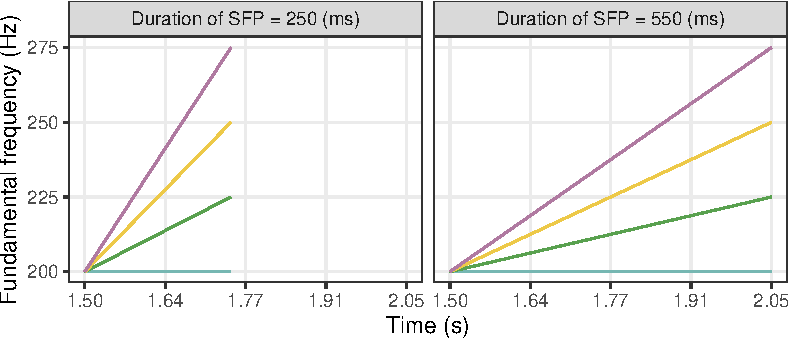
\includegraphics[width=10cm]{figures/stimuli.pdf}
    \caption{Schematic representation of some manipulations.}
    \label{fig:stimuli}
\end{figure}

\subsection{Procedure}\label{subsubsec:procedure}

Seventeen native speakers of Cantonese took part in the experiment. In each trial, after listening to the stimulus, the participant completed a three-alternative forced choice task, with each option exemplifying one of the three readings. For instance, upon hearing an utterance like \xref{stimulus}, with a prosodically manipulated sentence-final particle, the participant had to pick one of the three options shown in \xref{3AFC} that they thought matched the intonation of the utterance.

\begin{exe}
\let\eachwordone=\cn
\ex\label{3AFC}
\begin{xlist}
\ex\label{3AFC1} \glll 講嘢嘅人 唔 知道 邊個 想 飲 咖啡 (ISQ) \\
gong\textsuperscript{2}je\textsuperscript{5}ge\textsuperscript{3}jan\textsuperscript{4} m\textsuperscript{4} zi\textsuperscript{1}dou\textsuperscript{3} bin\textsuperscript{1}go\textsuperscript{3} soeng\textsuperscript{2} jam\textsuperscript{2} gaa\textsuperscript{3}fe\textsuperscript{1} \\
speaker not know who want drink coffee \\
\trans `The speaker does not know who wants to drink coffee.'
\ex\label{3AFC2} \glll 講嘢嘅人 認為 冇人 想 飲 咖啡 (RQ$-$) \\
gong\textsuperscript{2}je\textsuperscript{5}ge\textsuperscript{3}jan\textsuperscript{4} jing\textsuperscript{6}wai\textsuperscript{4} mou\textsuperscript{5}jan\textsuperscript{4} soeng\textsuperscript{2} jam\textsuperscript{2} gaa\textsuperscript{3}fe\textsuperscript{1} \\
speaker think nobody want drink coffee \\
\trans `The speaker thinks nobody wants to drink coffee.'
\ex\label{3AFC3} \glll 講嘢嘅人 已經 知道 邊個 想 飲 咖啡 (RQ$+$) \\
gong\textsuperscript{2}je\textsuperscript{5}ge\textsuperscript{3}jan\textsuperscript{4} ji\textsuperscript{5}ging\textsuperscript{1} zi\textsuperscript{1}dou\textsuperscript{3} bin\textsuperscript{1}go\textsuperscript{3} soeng\textsuperscript{2} jam\textsuperscript{2} gaa\textsuperscript{3}fe\textsuperscript{1} \\
speaker already know who want drink coffee \\
\trans `The speaker already knows who wants to drink coffee.'
\end{xlist}
\end{exe}

\subsection{Analysis}\label{subsubsec:analysis}

Given that there were three possible responses for each trial, we employed a Bayesian multilevel multinomial logistic regression, with a random intercept for each participant but shared fixed effects for all participants \citep{Koster+2017}. The reference level for the dependent variable was the information-seeking question response. Alongside the intercept, the predictor variables included duration and pitch rise, both of which were \textit{z}-transformed before entering the analysis. The priors for all coefficients were a normal distribution with a mean of 0 and a standard deviation of 1. For the correlation structure of the random intercept, a zero-mean multivariate normal distribution was used with an exponential distribution with rate 1 and an LKJ distribution with $\xi = 2$ as the priors for the standard deviation and the correlation matrix associated with the covariance matrix.

\subsection{Results}\label{subsubsec:results}

%The proportions for each response type under different duration and pitch conditions are shown in Figures \ref{fig:ret1} and \ref{fig:ret2}.

Overall, the model confirms that different combinations of pitch contours and duration on the sentence-final particle led to different proportions of information-seeking, empty set, and non-empty set rhetorical question responses. Specifically, the model results suggest that, relative to information-seeking question responses, a longer duration led to both more empty set (95\% credible interval [CrI] $= [0.33, 0.47]$) and non-empty set rhetorical question responses (95\% CrI $= [0.39, 0.60]$), even though the posterior predictive pattern for non-empty set rhetorical questions does not show a clear trend (see \figref{fig:ret1}).

\begin{figure}
    \centering
    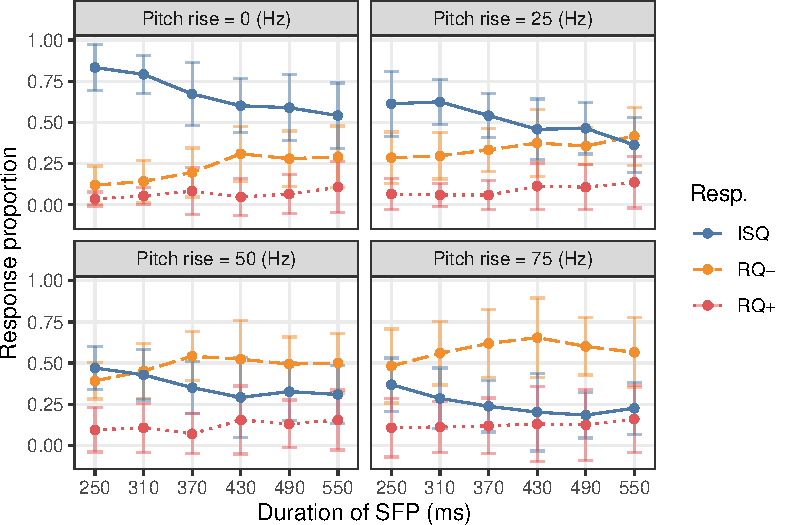
\includegraphics[width=11cm]{figures/results_duration_no_tag.pdf}
    \caption{Response proportions of information-seeking questions (ISQ), empty set rhetorical questions (RQ$-$) and non-empty set rhetorical questions (RQ$+$) as a function of manipulated duration.}
    \label{fig:ret1}
\end{figure}

With respect to pitch rise, again a larger pitch rise led to more empty set (95\% CrI $= [0.66, 0.80]$) and non-empty set rhetorical question responses (95\% CrI $= [0.59, 0.80]$), although the trend for non-empty set rhetorical question responses is not as clear (see \figref{fig:ret2}).

\begin{figure}
    \centering
    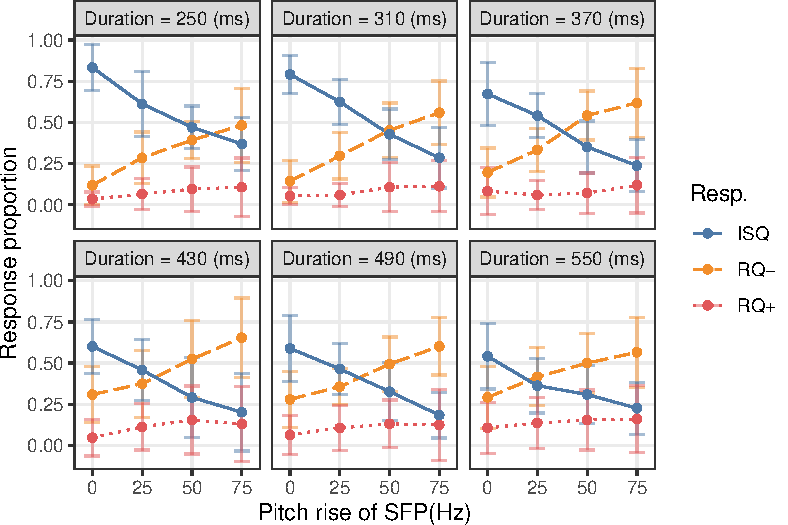
\includegraphics[width=11cm]{figures/results_pitch_no_tag.pdf}
    \caption{Response proportions of information-seeking questions (ISQ), empty set rhetorical questions (RQ$-$), and non-empty set rhetorical questions (RQ$+$) as a function of manipulated pitch rise.}
    \label{fig:ret2}
\end{figure}

\subsection{Discussion}

The results of the perception experiment do not entirely conform the results of the production experiment of \citet{Lo+2019}. While the prosodic cues participants associated with information-seeking questions were similar to the prosodic cues of this question type in production (a lower, non-rising pitch and a relatively short duration, see \tabref{tab:Loetal}), rhetorical questions showed some novel patterns. Namely, empty set rhetorical questions (RQ$-$), which were produced with a low and level pitch, were associated with a rising contour in perception. And rhetorical questions with a non-empty set as answer (RQ$+$), which were produced with a rising pitch, were not clearly associated with any pitch contour, as shown in \figref{fig:ret1}. 

As for duration, \figref{fig:ret1} shows us that regardless of pitch, the longer the sentence-final particle is, the more likely speakers are to interpret the utterance as an empty set rhetorical question. This is a contrast that was also found to be significant in production (see \tabref{tab:Loetal}). Cantonese wh-questions with the particle \textit{aa\textsuperscript{3}} thus provide a further example for the observations made in other languages (see \sectref{subsec:previous}) that boundary tones are not sufficient in characterizing the prosody of information-seeking and rhetorical questions.

In general, a three-way distinction between information-seeking questions, empty set and non-empty set rhetorical questions was found, as in production, even if the three particular forms were somewhat different in production and perception. While we do not know why there was only a partial match between the production and perception of the specific pitch contours, the three way contrast found in both cases can be interpreted as a support for there being a three-way contrast in meaning.


%The fact that only information-seeking questions and empty set rhetorical questions got associated with a certain pitch contour is particularly interesting in light of their semantic properties. 

\section{General discussion}
\label{sec:discussion}

The results of our experiment confirm that there is a three-way distinction in form between information-seeking, empty set and non-empty set rhetorical questions. These results thus support our proposal for the semantics of these question types.

In addition to that, we posited a conditional prediction that in case there is a three-way distinction, those question types that depend less on the context (i.e., that do not depend on the common ground) in order to be interpreted as intended would be associated with certain prosodic forms more strongly than those that do rely on the common ground. This prediction, too, is borne out: as \figref{fig:ret1} and \figref{fig:ret2} show, only information-seeking questions and empty set rhetorical questions were clearly associated with a certain combination of prosodic cues.

We argue that this tendency is explained by an inquisitive semantic analysis. We proposed in \sectref{subsec:gradient} that information-seeking questions, non-empty set rhetorical questions and empty set rhetorical questions form a scale in terms of inquisitiveness and informativity. On the inquisitive end of the scale, we find information-seeking questions which are inquisitive and not at all informative. Considering questions only, on the informative end of the scale we find empty set rhetorical questions, which are both inquisitive and informative. And between the two are rhetorical questions with a non-empty answer, which are also both inquisitive and informative, but which are less informative than the ones with an empty set answer.

We have argued that these properties map to different levels of context-depen-dence and that there is an asymmetry between the two types of rhetorical questions. If the suggested answer is the empty set, the addressee receives the issue already resolved and there is no need to consult the common ground. This is not the case if the rhetorical question suggests a non-empty answer, which the addressee can only resolve by consulting the common ground. The intended answer itself is not directly encoded by virtue of the marked form of the utterance; it therefore remains highly context-dependent, a property that led \citet{Jamieson2018phd} to call them ``pragmatic'' rhetorical questions. Information-seeking questions, which are inquisitive and not informative, are again less dependent on the context compared to non-empty set rhetorical questions in the sense that the addressee does not need the common ground in order to arrive at the intended interpretation of the utterance. 

In sum, only those utterance types which are relatively context-independent have been associated with a clear prosodic pattern: information-seeking questions and empty set rhetorical questions. The explanation we offer is that the utterance types that can be interpreted more independently from the context are also the ones that are more likely to conventionalize their prosodic cues. And if prosodic cues become conventionalized, it explains why participants associated them more strongly with the relevant question types. The reason why non-empty set rhetorical questions were not associated with a certain intonational pattern is because they convey context-sensitive information, namely, they intend to point to an already known answer. But which member(s) of the domain it points to is not grammatically encoded, simply because there is no straightforward way to do so. 

%We suggest that since both information-seeking questions and empty set rhetorical questions are interpretable without knowing the common ground, they developed their own intonational contours which addressees can rely on when interpreting these utterances. The interpretation of non-empty set rhetorical questions, on the other hand, is highly dependent on the common ground, and the proposed answer is therefore not stabile across contexts; and if this is the case, the answer cannot be encoded by an intonational pattern.

As for the mismatch between our production and perception results, we are not in a position to establish straightforward form-meaning mappings for the three wh-question types in Cantonese. The form-meaning relations that we propose here are at a more abstract level, so further research is needed to explore the durational and pitch properties of the sentence-final particle \textit{aa\textsuperscript{3}} in the three question types. We speculate that the mismatch found between the production and perception results may be due to perceiving the sentence-final particle as \textit{aa\textsuperscript{1}}, especially in empty set rhetorical questions, even though instead of a high level tone, it got associated with a rising contour,  which is closest to the high level tone of this particle in terms of its pitch. Cantonese sentence-final particles usually come in families: the same segmental material can wear multiple tones, each of which alters its meaning. So even though intonation has been shown to completely override the lexical tone found on the last syllable of the utterance, we cannot exclude the possibility that the tonal differences between \textit{aa\textsuperscript{3}} and \textit{aa\textsuperscript{1}} had no effect on the dependent variable.

In addition, the mismatch between production and perception may also be due to prosodic cues that were not included here as independent variables. On the one hand, breathy voice has been shown to be a marker of German rhetorical questions in production \citep{Braun+2018}, and the role of intensity in either producing or processing the three utterance types remains unexplored. Considering these cues in future perception experiments may therefore be advantageous. On the other hand, the fact that all stimuli were produced from utterances that were meant to be information-seeking questions may also have played an important role. Even though \citet{Lo+2019} only found significant differences between the prosodic realization of the sentence-final particles of the three question types, further prosodic cues may have characterized the rest of the utterance, which may have affected perception of our stimuli.


As far as the validity of our analysis is concerned, the results of our experiment not only support our analysis but that of \citet{Jamieson2018phd} as well. In his account, too, ``generic'' and ``pragmatic'' rhetorical questions differ in how much the addressee has to rely on the context (namely on the common ground) in order to interpret the question. It is not the goal of this paper to evaluate \citeauthor{Jamieson2018phd}'s account, however; comparing it to the account offered here is left for future work. For now we can only point to one advantage, namely that the ``generic'' and ``pragmatic'' nature of empty set and non-empty set rhetorical questions follows from our inquisitive semantic analysis, without having to posit a metavariable in order to derive the meaning of empty set rhetorical questions.

\section{Conclusion}
\label{sec:conclusion}

In this paper, we have argued that when analyzing the meaning of rhetorical questions, the kind of answer they suggest plays an important role in their meaning. Information-seeking questions commit the speaker to all alternatives, empty set rhetorical questions, to the empty set alternative, and non-empty set rhetorical questions, to $\Alpha$, all alternatives except the empty set one. We presented experimental results that we take as a support to this claim. First, a three-way prosodic distinction has been found between these three question types. Second, participants clearly associated information-seeking and empty set rhetorical questions with certain forms. These utterance types are on the two edges of the informative/inquisitive scale of interrogatives, and as such, they have a meaning that generalizes across contexts, as opposed to non-empty set rhetorical questions, which remain context-sensitive.

The question of what the intonational contours of the sentence-final particles in rhetorical questions really look like remains open, along with the question of what other prosodic cues not mentioned here may play a role in shaping the intonation of information-seeking and rhetorical questions in Cantonese. But the claims made here are nevertheless falsifiable and have cross-linguistic relevance, and as such, they invite further work on rhetorical questions.

\section*{Acknowledgements}
We thank Lisa Cheng, Beáta Gyuris, E Jamieson, Zoe Lam, Michela Ippolito, Pilar Prieto, Floris Roelofsen, Tue Trinh and Maxime Tulling; the audiences at International Congress of Phonetic Sciences (2019), the Annual Conference of the Canadian Linguistic Association (2019), Laboratory, Phonology 17, Sinn und Bedeutung 25, LSA95, the workshop \textit{Biased Questions: Experimental Results \& Theoretical Modelling}, and the 4th Forum on Cantonese Linguistics; as well as all our participants.

\printbibliography[heading=subbibliography, notkeyword=this]

\end{document}
